% =====================================================================
%  CLASE 06 -- Pruebas de bombeo
% =====================================================================
\clase{06}{Pruebas de bombeo}

\section{Resumen}
\begin{table}[H]
\centering
\renewcommand{\arraystretch}{2.2}
\begin{tabular}{l>{$\displaystyle}c<{$}}
\toprule
\textbf{Caso} & \textbf{Ecuación}\\
\midrule
Penetración total, acuífero confinado & \Delta h=H-h=\frac{Q}{2\pi T}\ln\left(\frac Rr\right)\\
Penetración total, acuífero libre & H^2-h^2=\frac{Q}{\pi K}\ln\left(\frac Rr\right)\\
Acuífero artesiano, impermanente & \Delta h=H-h=\frac{Q}{2\pi T}\ln\left(\frac{R(t)}{r}\right)\\
Acuífero libre, impermanente & H^2-h^2=\frac{Q}{\pi K}\ln\left(\frac{R(t)}{r}\right)\\
Radio de influencia transiente & R(t)=\sqrt{\frac{2.24\cdot T\cdot t}{S}}\\
\bottomrule
\end{tabular}
\end{table}

\section{Pruebas de bombeo}
\begin{itemize}
  \item Para determinar parámetros del acuífero ($K$, $S$).
  \item Extracción de agua y control de niveles en el pozo.
  \item En condiciones de equilibrio y desequilibrio.
  \item Cálculo del comportamiento a largo plazo de un pozo.
  \item Cálculo del radio de protección de un pozo (para derechos de agua, por ejemplo).
  \item Ideal contar con pozos de observación.
  \item Generalmente las pruebas se realizan en el mismo pozo, por lo que los
        resultados presentan incertidumbre.
\end{itemize}

\begin{figure}[H]
\centering
\begin{tikzpicture}[font=\scriptsize,scale=1.0]
  \fill[suelo!60] (0,0) rectangle (9,0.4); \node at (1.2,0.2) {Basamento};
  \fill[aguaclara] (0,0.4) rectangle (9,2.6);
  \fill[sueloclaro] (0,2.6) -- (9,2.6) -- (9,3.3) -- (0,3.3) -- cycle;
  \fill[aguaclara] (0,2.6) -- (0,2.4) .. controls (2,2.3) and (3,1.3) .. (3.4,1.2) -- (3.8,1.2) .. controls (4.2,1.3) and (6,2.3) .. (9,2.4) -- (9,2.6) -- cycle;
  \fill[sueloclaro] (0,2.4) .. controls (2,2.3) and (3,1.3) .. (3.4,1.2) -- (3.8,1.2) .. controls (4.2,1.3) and (6,2.3) .. (9,2.4) -- (9,2.6) -- (0,2.6) -- cycle;
  \draw[dashed,azulusm,thick] (0,2.6) -- (9,2.6);
  \draw[azulusm,thick] (0,2.4) .. controls (2,2.3) and (3,1.3) .. (3.4,1.2) -- (3.8,1.2) .. controls (4.2,1.3) and (6,2.3) .. (9,2.4);
  \draw (0,3.3) -- (9,3.3);
  \fill[white,draw] (3.4,0.4) rectangle (3.8,3.9); \fill[agua] (3.4,0.4) rectangle (3.8,1.2);
  \fill[white,draw] (6.4,0.8) rectangle (6.6,3.9); \fill[agua] (6.4,0.8) rectangle (6.6,2.2);
  \draw[flecha,azulusm] (3.6,1.4) -- (3.6,4.3) -- (2.8,4.3) node[left,black]{Caudal de bombeo};
  \node[above] at (3.6,4.4) {Pozo de bombeo};
  \node[above,align=center] at (6.5,3.9) {Pozo de\\observación};
  \draw[cota] (7.0,2.2) -- (7.0,2.6) node[midway,right]{Descenso};
  \node[right,align=left] at (7.3,3.0) {Nivel estático original};
  \draw[<-] (2.2,1.9) -- (1.2,1.3) node[below,align=center]{Nivel de agua luego\\del bombeo};
  \draw[<-] (2.8,1.6) -- (1.0,3.7) node[above]{Cono de depresión};
  \node at (5,0.9) {Acuífero};
\end{tikzpicture}
\caption{Esquema de una prueba de bombeo con pozo de observación.}
\end{figure}

\subsection{Solicitud de derecho subterráneo (DGA)}
Según la \emph{Guía para la presentación de Solicitudes de Derechos de
Aprovechamiento de Aguas Subterráneas} (DGA, versión 25.05.2022), los
antecedentes técnicos mínimos son:
\begin{itemize}
  \item \textbf{Pozos profundos y punteras:} perfil estratigráfico;
        habilitación; \textbf{prueba de bombeo de gasto constante} para el
        caudal solicitado, con una duración de 24 horas como mínimo y con un
        tiempo de estabilización de niveles de 180 minutos (sin perjuicio de
        otros antecedentes, como una prueba de gasto variable, si la hubiere);
        los datos de recuperación completa de la obra, o hasta que se haya
        estabilizado la recuperación.
  \item \textbf{Norias y drenes:} prueba de bombeo de gasto constante para el
        caudal solicitado, con estabilización de niveles de por lo menos 180
        minutos; para drenes podrían requerirse registros de caudales medidos
        mediante aforos; para norias, los datos de recuperación completa de la obra.
  \item \textbf{Pozos zanjas:} prueba de bombeo de gasto constante para el
        caudal solicitado durante 24 horas, con estabilización de niveles de
        por lo menos 180 minutos; perfil estratigráfico y dimensiones de la obra.
\end{itemize}

\section{Prueba de gasto variable}
\begin{itemize}
  \item Para determinar el caudal máximo a extraer del pozo y la ubicación de la bomba.
  \item Se aumenta paulatinamente el caudal bombeado.
  \item Para cada caudal, se deja estabilizar el sistema.
  \item Si el acuífero es artesiano se obtiene una recta (uniendo los puntos
        de estabilización de cada escalón); si es libre, se puede linealizar el problema.
\end{itemize}

\begin{figure}[H]
\centering
\begin{tikzpicture}
\begin{axis}[width=10cm,height=6cm,xmin=0,xmax=18,ymin=0,ymax=25,
  xlabel={Tiempo [h]},ylabel={Descenso [m]},grid=major,grid style={dashed,gray!40}]
  \addplot[thick,black] coordinates {(0,0)(0.1,3)(0.5,4)(3,4.5)};
  \addplot[thick,red] coordinates {(3,4.5)(3.1,5.8)(3.5,6.2)(6,6.5)};
  \addplot[thick,green!60!black] coordinates {(6,6.5)(6.1,8.5)(6.5,9)(9,9.3)};
  \addplot[thick,blue] coordinates {(9,9.3)(9.1,12)(9.5,12.7)(12,13)};
  \addplot[thick,magenta] coordinates {(12,13)(12.1,16)(12.5,16.6)(15,17)};
  \addplot[thick,green!40!black] coordinates {(15,17)(15.1,20.5)(15.5,21.5)(18,22)};
  \addplot[very thick,dashed,azulusm] coordinates {(3,4.5)(6,6.5)(9,9.3)(12,13)(15,17)(18,22)};
\end{axis}
\end{tikzpicture}
\caption{Prueba de gasto variable (escalonada): descenso versus tiempo.}
\end{figure}

\section{Prueba de gasto constante}
\begin{itemize}
  \item Para determinar los parámetros elásticos del acuífero ($K$, $S$).
  \item En Chile se realizan por 24 horas, con 3 horas de estabilización.
  \item Se realiza para el 80\% del $Q$ máximo de la prueba de gasto variable.
\end{itemize}

\paragraph{Prueba de recuperación}
\begin{itemize}
  \item En un tiempo $t_f$ se deja de bombear, para que los niveles se recuperen.
  \item Permite la determinación de $K$.
\end{itemize}

\begin{figure}[H]
\centering
\begin{subfigure}{0.48\textwidth}\centering
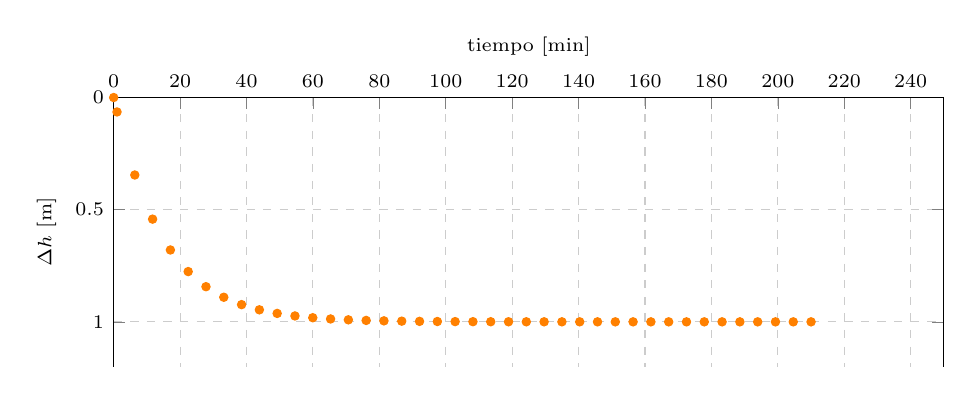
\begin{tikzpicture}
\begin{axis}[width=\linewidth,height=5cm,xmin=0,xmax=250,ymin=0,ymax=1.2,y dir=reverse,
  axis x line*=top,xlabel={tiempo [min]},ylabel={$\Delta h$ [m]},grid=major,grid style={dashed,gray!40},font=\scriptsize]
  \addplot[only marks,mark=*,orange,mark size=1.5pt,domain=1:210,samples=40] {1.0*(1-exp(-x/15))};
  \addplot[only marks,mark=*,orange,mark size=1.5pt] coordinates {(0,0)};
\end{axis}
\end{tikzpicture}
\caption{Descenso en prueba de gasto constante.}
\end{subfigure}\hfill
\begin{subfigure}{0.48\textwidth}\centering
\begin{tikzpicture}[font=\small]
  \draw[flecha] (0,0) -- (5,0) node[right]{$t$};
  \draw[flecha] (0,0) -- (0,-2.6) node[left]{$\Delta h$};
  \draw[orange,very thick,dashed] (0,0) .. controls (0.5,-1.5) and (1.5,-1.8) .. (3,-1.95);
  \draw[orange,very thick] (3,-1.95) .. controls (3.3,-1.2) and (3.6,-0.8) .. (4.9,-0.3);
  \draw[dashed] (3,0.3) node[above]{$t_f$} -- (3,-2.2);
\end{tikzpicture}
\caption{Prueba de recuperación a partir de $t_f$.}
\end{subfigure}
\caption{Prueba de gasto constante y prueba de recuperación.}
\end{figure}

\section{Interpretación de la prueba de gasto constante}

\subsection{Método de la curva tipo (Theis)}
Solución gráfica propuesta por Theis. Como $u$ es sensible para valores de
$t$ pequeños, se definen dos soluciones aproximadas distintas de $W(u)$ con
más detalle, por medio de series de Taylor:
\begin{itemize}
  \item Para $u<1$:
  \begin{formula}
  $W(u)=u-0.2499u^2+0.0552u^3-0.0098u^4+0.00108u^5-\ln(u)-0.5772$
  \end{formula}
  \item Para $u\geq1$:
  \begin{formula}
  $\displaystyle W(u)=\frac{mH_1}{nH_1\cdot u\cdot e^u}$
  \end{formula}
  donde
  \[
  mH_1=u^4+8.573u^3+18.059u^2+8.635u+0.268,
  \]
  \[
  nH_1=u^4+9.573u^3+25.633u^2+21.097u+3.958
  \]
\end{itemize}

\paragraph{Procedimiento}
\begin{enumerate}
  \item Graficar $W(u)$ en función de $1/u$ (ejes logarítmicos).
  \item Graficar la depresión en el pozo en función del tiempo (ejes logarítmicos, misma escala).
  \item Mover los gráficos en dirección horizontal y vertical, hasta que los
        datos teóricos se ubiquen sobre los datos de terreno. ¡Cuidado de no
        girar los gráficos!
  \item Una vez conseguido el mejor ajuste, se selecciona un punto en el
        gráfico y se determina el valor de los 4 ejes: $W(u)$, $1/u$,
        $\Delta h^*$ y $t^*$.
  \item Con estos valores se determinan los parámetros del acuífero:
\end{enumerate}
\begin{formula}
$\displaystyle T=\frac{Q}{4\cdot\pi\cdot\Delta h^*}\cdot W(u)\qquad\qquad
S=\frac{4\cdot T\cdot u\cdot t^*}{r^2}$
\end{formula}
¡Imprescindible para tiempos de bombeo pequeños!

\begin{figure}[H]
\centering
\begin{tikzpicture}
\begin{loglogaxis}[width=10cm,height=7cm,xmin=0.1,xmax=1e4,ymin=0.01,ymax=10,
  xlabel={$1/u$},ylabel={$W(u)$},grid=both,minor grid style={gray!15},major grid style={gray!40},
  clip=false]
\addplot[thick,orange] coordinates {(0.3162,0.01063) (0.3981,0.02453) (0.5012,0.04922) (0.631,0.08824) (0.7943,0.1444) (1,0.2194) (1.259,0.3138) (1.585,0.4272) (1.995,0.5583) (2.512,0.7056) (3.162,0.867) (3.981,1.041) (5.012,1.225) (6.31,1.417) (7.943,1.617) (10,1.823) (12.59,2.034) (15.85,2.248) (19.95,2.466) (25.12,2.686) (31.62,2.908) (39.81,3.132) (50.12,3.357) (63.1,3.583) (79.43,3.81) (100,4.038) (125.9,4.266) (158.5,4.495) (199.5,4.724) (251.2,4.953) (316.2,5.182) (398.1,5.412) (501.2,5.642) (631,5.872) (794.3,6.102) (1000,6.332) (1259,6.562) (1585,6.792) (1995,7.022) (2512,7.252) (3162,7.482) (3981,7.712) (5012,7.943) (6310,8.173) (7943,8.403) (1e+04,8.633)};
\addplot[only marks,mark=o,azulusm,mark size=1.3pt] coordinates {(5,1.2)(8,1.6)(12,2.0)(20,2.45)(30,2.9)(50,3.35)(80,3.8)(120,4.2)(200,4.7)(300,5.1)(500,5.6)(800,6.1)(1200,6.5)(2000,7.0)};
\draw[dashed,rojo,thick] (axis cs:0.1,4.7) -- (axis cs:200,4.7) -- (axis cs:200,0.01);
\fill[rojo] (axis cs:200,4.7) circle (2pt);
\node[rojo,above] at (axis cs:200,5.2) {Punto elegido};
\node[rojo,left] at (axis cs:0.1,4.7) {$W(u)$, $\Delta h^*$};
\node[rojo,below] at (axis cs:200,0.01) {$1/u$, $t^*$};
\end{loglogaxis}
\end{tikzpicture}
\caption{Método de la curva tipo: superposición de las mediciones ($\Delta h$
vs.\ $t$, puntos) sobre la curva de Theis ($W(u)$ vs.\ $1/u$) y elección de un
punto de ajuste.}
\end{figure}

\subsection{Método de Cooper--Jacob (1946)}
\begin{itemize}
  \item Graficar los datos de terreno en papel semilog ($\Delta h$ vs.\ $\ln t$).
  \item Las constantes del acuífero se obtienen a partir del ajuste lineal.
  \item Se deben cumplir las hipótesis de Jacob ($u$ pequeño).
\end{itemize}
\begin{formula}
$\displaystyle T=\frac{Q}{4\cdot\pi\cdot a}\qquad a$: pendiente de la recta\\[6pt]
$\displaystyle S=\frac{2.24\cdot T\cdot t_0}{r^2}\qquad t_0$: punto artificial donde $\Delta h=0$
\end{formula}

\begin{figure}[H]
\centering
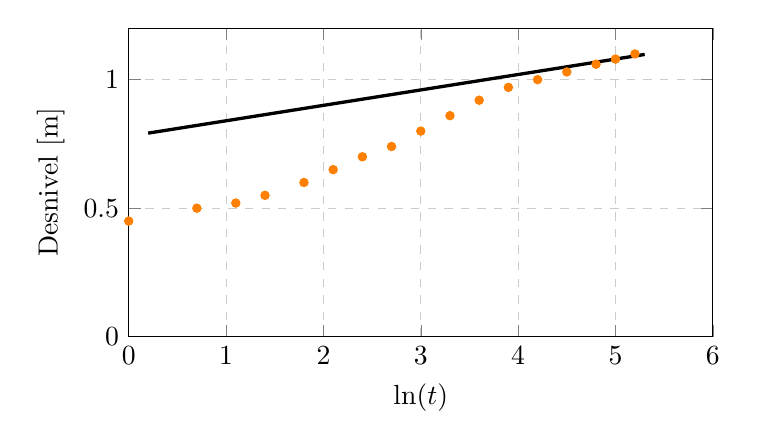
\begin{tikzpicture}
\begin{axis}[width=9cm,height=5.5cm,xmin=0,xmax=6,ymin=0,ymax=1.2,
  xlabel={$\ln(t)$},ylabel={Desnivel [m]},grid=major,grid style={dashed,gray!40}]
  \addplot[only marks,mark=*,orange,mark size=1.5pt] coordinates {(0,0.45)(0.7,0.5)(1.1,0.52)(1.4,0.55)(1.8,0.6)(2.1,0.65)(2.4,0.7)(2.7,0.74)(3.0,0.8)(3.3,0.86)(3.6,0.92)(3.9,0.97)(4.2,1.0)(4.5,1.03)(4.8,1.06)(5.0,1.08)(5.2,1.1)};
  \addplot[very thick,black,domain=0.2:5.3] {0.78+0.06*x};
\end{axis}
\end{tikzpicture}
\caption{Método de Cooper--Jacob: ajuste lineal en papel semilogarítmico.}
\end{figure}

\subsection{Método de Papadopulos--Cooper}
\begin{itemize}
  \item Útil para pozos de gran diámetro.
  \item No es posible despreciar el almacenamiento de agua dentro del pozo.
\end{itemize}
En régimen transiente se cumple $Q\neq Q_B$ con $Q_B>Q$. Considerando el
volumen de control definido por el pozo:
\[
Q_i-Q_s=\frac{\partial V}{\partial t}\;\Rightarrow\;Q_i-Q_s=\pi r_0^2\frac{\partial h_0}{\partial t}
\]
Por otro lado, considerando
\[
\frac{\partial^2h}{\partial r^2}+\frac1r\frac{\partial h}{\partial r}=\frac ST\frac{\partial h}{\partial t}
\]
con $r_0$: radio efectivo del pozo (entubación) y $r$: radio de habilitación
del pozo (incluye el filtro de grava). Se obtiene:
\begin{formula}
$\displaystyle\Delta h=\frac{Q}{4\cdot\pi\cdot T}\cdot W(u,\alpha),\qquad
u=\frac{r^2\cdot S}{4\cdot T\cdot t},\qquad\alpha=S\cdot\left(\frac{r_0}{r}\right)^2$
\end{formula}
¡Similar a Theis, se puede utilizar el método de la curva tipo (una curva
por cada valor de $\alpha$)!

\subsection{Método de Hantush--Jacob (1955)}
\begin{itemize}
  \item Acuífero semi-confinado, de pequeño diámetro.
  \item Desprecia el almacenamiento de agua dentro del pozo.
\end{itemize}
Resolvió la siguiente ecuación diferencial (con $s$ el descenso, $K'$ y $m'$
la conductividad y espesor de la capa semiconfinante):
\[
\frac{\partial^2s}{\partial r^2}+\frac1r\frac{\partial s}{\partial r}-\frac{K'}{Tm'}s=\frac ST\frac{\partial s}{\partial t}
\]
obteniendo:
\begin{formula}
$\displaystyle\Delta h=\frac{Q}{4\cdot\pi\cdot T}\cdot W\!\left(u,\frac rB\right),\qquad
u=\frac{r^2\cdot S}{4\cdot T\cdot t},\qquad B=\sqrt{\frac{T\cdot m'}{K'}}$
\end{formula}
¡Similar a Theis, se puede utilizar el método de la curva tipo (familia de
curvas para distintos $r/B$)!

\begin{figure}[H]
\centering
\begin{tikzpicture}[font=\small,scale=0.9]
  \draw[thick] (-4,0) -- (4,0);
  \foreach \x in {-3.9,-3.6,...,3.9} \draw (\x,0) -- (\x-0.2,-0.25);
  \fill[pattern=north east lines] (-4,2.0) rectangle (-0.4,2.4);
  \fill[pattern=north east lines] (0.4,2.0) rectangle (4,2.4);
  \draw (-4,2.0) -- (-0.4,2.0) (0.4,2.0) -- (4,2.0) (-4,2.4) -- (-0.4,2.4) (0.4,2.4) -- (4,2.4);
  \foreach \x in {-3.5,-3.0,...,-1.0,1.0,1.5,...,3.5} \draw[->,rojo] (\x,2.9) -- (\x,2.05);
  \draw[thick] (-0.4,0) -- (-0.4,4.2) (0.4,0) -- (0.4,4.2);
  \draw[thick] (-4,4.2) -- (-0.4,4.2) (0.4,4.2) -- (4,4.2);
  \draw[dashed,cyan!70!blue,thick] (-4,3.7) -- (-0.4,3.7) (0.4,3.7) -- (4,3.7) node[right]{$t=0$};
  \draw[cyan!70!blue,thick] (-4,3.4) .. controls (-2,3.3) and (-1,2.8) .. (-0.4,2.5) -- (0.4,2.5) .. controls (1,2.8) and (2,3.3) .. (4,3.4) node[right]{$t=t$};
  \fill[azulusm] (-0.1,4.1) rectangle (0.1,4.7); \fill[azulusm] (-0.25,4.7) -- (0.25,4.7) -- (0,5.0) -- cycle; \node at (0.5,4.9) {$Q_s$};
  \draw[cota] (-3.3,0) -- (-3.3,2.0) node[midway,left]{$m$};
  \draw[cota] (-4.3,2.0) -- (-4.3,2.4) node[midway,left]{$m'$};
  \node at (-2.2,1.0) {$K,S$}; \node at (-1.5,2.2) [fill=white,inner sep=1pt]{$K'$};
  \node[azulusm,font=\scriptsize] at (2.3,1.7) {Capa confinante};
  \draw[->,azulusm] (1.5,1.0) -- (0.5,1.0) node[pos=0,right]{$Q_i$};
\end{tikzpicture}
\caption{Pozo en acuífero semiconfinado (Hantush--Jacob): filtración vertical a través del acuitardo.}
\end{figure}

\subsection{Acuíferos libres}
Para acuíferos libres se puede usar la linealización del problema:
\begin{itemize}
  \item El método gráfico original no es válido; hay modificaciones (se
        considera el drenaje diferido).
  \item Sí es válido el método de Jacob.
  \item La prueba de recuperación es válida.
\end{itemize}
\begin{formula}
$\displaystyle\Delta h'=\Delta h-\frac{(\Delta h)^2}{2H},\qquad
\Delta h'=\frac{Q}{4\cdot\pi\cdot K\cdot H}\ln\left(\frac{2.24\cdot T\cdot t}{S\cdot r^2}\right)$
\end{formula}
Tener cuidado si existen recargas o barreras impermeables en las cercanías del pozo.

\section{Interpretación de la prueba de recuperación}
\begin{itemize}
  \item Puede modelarse por superposición: a partir de $t_f$ se agrega un
        pozo imagen ficticio que inyecta $-Q$ en el mismo lugar.
  \item Debe respetar el supuesto de Jacob.
  \item Para la zona de recuperación se grafica $\Delta h$ vs.\
        $\ln\frac{t}{t-t_f}$; la parte inicial es una recta.
  \item ¡Similar a Theis, se puede utilizar el método de la curva tipo!
\end{itemize}

\begin{figure}[H]
\centering
\begin{tikzpicture}[font=\small]
  \draw[flecha] (0,0) -- (6,0) node[right]{$t$};
  \draw[flecha] (0,1.2) -- (0,-2.6) node[left]{$\Delta h$};
  \node[left] at (0,1.0) {$Q$};
  \fill[gray!20,draw] (0,0) rectangle (5.8,0.4); \node[left] at (0,0.4) {$+Q$};
  \fill[gray!20,draw] (3.5,0) rectangle (5.8,-0.4); \node[right] at (5.8,-0.4) {$-Q$};
  \draw[orange,very thick,dashed] (0,0) .. controls (0.5,-1.5) and (1.5,-1.9) .. (3.5,-2.1);
  \draw[orange,very thick] (3.5,-2.1) .. controls (3.8,-1.3) and (4.2,-0.9) .. (5.8,-0.5);
  \draw[dashed] (3.5,0.6) node[above]{$t_f$} -- (3.5,-2.3);
\end{tikzpicture}
\caption{La recuperación se modela superponiendo un caudal $-Q$ desde $t_f$.}
\end{figure}

\section{Pruebas de bombeo con condiciones de borde}

\subsection{Barrera impermeable}
Se utiliza el método de las imágenes. En el gráfico $\Delta h$ vs.\ $\ln t$
la pendiente se \textbf{duplica} cuando el pozo imagen comienza a afectar.
\begin{itemize}
  \item Estimar los parámetros del acuífero con la parte no perturbada del gráfico.
  \item Es posible estimar la distancia hasta la barrera.
\end{itemize}

\subsection{Recarga lineal}
Se utiliza el método de las imágenes. En el gráfico $\Delta h$ vs.\ $\ln t$
la curva se \textbf{estabiliza} (pendiente nula) cuando el pozo imagen
comienza a afectar.
\begin{itemize}
  \item Estimar los parámetros del acuífero con la parte no perturbada del gráfico.
  \item Es posible estimar la distancia hasta la fuente de recarga.
\end{itemize}

\begin{figure}[H]
\centering
\begin{subfigure}{0.48\textwidth}\centering
\begin{tikzpicture}[font=\small]
  \draw[flecha] (0,0) -- (5,0) node[right]{$\ln(t)$};
  \draw[flecha] (0,0) -- (0,-3.5) node[left]{$\Delta h$};
  \draw[azulusm,thick] (0,0) -- (2.8,-1.4) -- (4.2,-3.2);
  \draw[azulusm,dashed] (2.8,-1.4) -- (4.8,-2.4);
  \draw[cota] (1.2,0) -- (1.2,-0.6) node[midway,right]{$\Delta h_1$};
  \node[above] at (1.2,0) {$\ln(t_1)$};
  \draw[dashed] (3.9,0) node[above]{$\ln(t_2)$} -- (3.9,-2.9);
  \draw[cota] (3.9,-1.95) -- (3.9,-2.8) node[midway,right]{$\Delta h_2$};
\end{tikzpicture}
\caption{Barrera impermeable.}
\end{subfigure}\hfill
\begin{subfigure}{0.48\textwidth}\centering
\begin{tikzpicture}[font=\small]
  \draw[flecha] (0,0) -- (5,0) node[right]{$\ln(t)$};
  \draw[flecha] (0,0) -- (0,-3.5) node[left]{$\Delta h$};
  \draw[azulusm,thick] (0,0) -- (2.6,-1.3) -- (4.8,-1.3);
  \draw[azulusm,dashed] (2.6,-1.3) -- (4.8,-2.4);
  \draw[cota] (1.2,0) -- (1.2,-0.6) node[midway,right]{$\Delta h_1$};
  \node[above] at (1.2,0) {$\ln(t_1)$};
  \draw[dashed] (4.2,0) node[above]{$\ln(t_2)$} -- (4.2,-2.2);
  \draw[cota] (4.2,-1.3) -- (4.2,-2.1) node[midway,right]{$\Delta h_2$};
\end{tikzpicture}
\caption{Recarga lineal.}
\end{subfigure}
\caption{Efecto de los bordes sobre la curva descenso--tiempo.}
\end{figure}

Si se tiene un pozo de observación a distancia $r_1$ del pozo de bombeo, se
eligen $t_1$ y $t_2$ tales que $\Delta h_1=\Delta h_2$ (desviación de la
recta igual a la depresión de la recta original):
\begin{formula}
$\displaystyle r_2=r_1\sqrt{\frac{t_2}{t_1}}\qquad\qquad d=\frac{r_1+r_2}{2}$
\end{formula}
donde $r_2$ es la distancia del pozo imagen al pozo de observación y $d$ la
distancia estimada al borde.
